\documentclass[a4paper,12pt]{article}

\usepackage[utf8]{inputenc}
\usepackage[czech]{babel}
\usepackage[IL2]{fontenc}
\usepackage[left=3cm,text={15cm, 23cm},top=3.5cm]{geometry}

\usepackage{graphicx}
\usepackage{tikz}

\usepackage{amssymb}
\usepackage{amsmath}
\usepackage{amsthm}
\usepackage{forest}
\usepackage[ruled,czech,linesnumbered,noline]{algorithm2e}
\usepackage{array}
\usepackage{multirow}
\usepackage{textcomp}
\usepackage{listings}

\usepackage{enumitem}

\usepackage{pgf}
\usepackage{tikz}
\usetikzlibrary{arrows,automata}

\newcounter{counten}
\setcounter{counten}{1}


\title{\bf PRL Projekt 3\,--\,Mesh multiplication}
\author{Vojtěch Havlena (xhavle03)}
\date{\today}

\begin{document}

\maketitle


\section{Rozbor a analýza algoritmu}
Algoritmus Mesh multiplication využívá $m\cdot k$ procesorů, uspořádaných do 2D mřížky, pro násobení matice $\mathbf{A}$ o rozměru 
$m\times n$ s maticí $\mathbf{B}$ o rozměru $n\times k$. Prvky matice $\mathbf{A}$ jsou postupně (zpožděně) posílány procesorům v 1. sloupci a  
prvky matice $B$ jsou posílány (zpožděně) procesorům v 1. řádku. Každý procesor $P_{i,j}$ obsahuje proměnnou $c_{ij}$, která
je na začátku nastavena na $0$. Na konci algoritmu je v proměnné $c_{ij}$ uložena hodnota výsledné matice na pozici $i,j$.

Algoritmus potom pracuje následovně. Jakmile procesor $P_{i,j}$ obdrží dvě hodnoty $a$ a $b$, do proměnné $c_{ij}$ uloží 
novou hodnotu $c_{ij} + a\cdot b$. Následně, jestliže $i < m$, procesor $P_{i,j}$ odesílá hodnotu $b$ procesoru 
$P_{i+1,j}$ (spodnímu sousedovi) a jestliže $j < k$, odesílá hodnotu $a$ procesoru $P_{i,j+1}$ (pravému sousedovi).
Tento postup se opakuje, dokud existují hodnoty $a$ a $b$, které byly poslány procesoru $P_{i,j}$.

\subsection*{Analýza složitosti}
Uvažujme, že algoritmus násobí matici $\mathbf{A}$ o rozměru $m\times n$ s maticí $\mathbf{B}$ o rozměru $n\times k$.
Algoritmus končí, jakmile procesor $P_{m,k}$ obdrží a zpracuje poslední hodnoty $a$ a $b$. Těmito hodnotami
jsou prvky $a_{m1}$ a $b_{1k}$. Díky zpoždění trvá $m+k+n-2$ kroků, než se tyto prvky dostanou do 
procesoru $P_{m,k}$. Časová složitost je tedy 
\begin{equation}
  t(m,k,n) = m+k+n-2 = \mathcal{O}(m+k+n).
\end{equation}
Vzhledem k tomu, že algoritmus pracuje na mřížce $m\times k$ procesorů, je počet procesorů (prostorová složitost)
možné vyjádřit jako $p(m,k,n) = m\cdot k$. Cena je tedy
\begin{equation}
  c(m,k,n) = t(m,k,n) \cdot p(m,k,n) =\mathcal{O}(m\cdot k\cdot (m+k+n)).
\end{equation}
V případě, že předpokládáme $m \leq n$ a $k\leq n$, dostáváme časovou složitost
\begin{equation}
  t(n) = \mathcal{O}(n).
\end{equation}
Při stejném předpokladu dostáváme prostorovou složitost $p(n) = n^2$ a 
celkovou cenu
\begin{equation}
  c(n) = t(n) \cdot p(n) = \mathcal{O}(n^3),
\end{equation}
která tedy není optimální.

\section{Implementace}
Algoritmus je implementován v jazyce C++ s využitím knihovny Open MPI. Jak již bylo zmíněno, implementace využívá $m\cdot k$ procesorů. 
Pro jednoduchost je v tomto textu použito označení procesorů $P_{i,j}$, kde $1 \leq i \leq m$, $1 \leq j \leq k$. Vzhledem k~tomu, 
že Open MPI přiřazuje identifikátory procesorům od 0 do $m\cdot k-1$, je označení $P_{i,j}$ pouze zkratka pro procesor s hodnotou 
Rank $(i-1)\cdot k+(j-1)$.

Před samotným algoritmem je procesorem $P_{1,1}$ provedeno načtení obou matic do paměti. Procesor $P_{1,1}$ provádí 
načítání, kontrolu a distribuci vstupních hodnot, stejně jako tisk výsledné matice, ale podílí se i na samotném algoritmu 
násobení matic. Následně procesor $P_{1,1}$ každému procesoru pošle hodnoty rozměrů matic ($m,n,k$) a krajním 
procesorů, t.j., procesorům $P_{i,1}$ a $P_{1,j}$, kde $1 \leq i \leq m$, $1 \leq j \leq k$ pošle odpovídající řádky a sloupce vstupních matic. Před začátkem 
algoritmu tedy krajní procesory mají v paměti tu část matice, kterou budou v samotném algoritmu postupně po 
jednotlivých prvcích posílat svým sousedům. Tato úvodní fáze není uvažována jak při odvozování teoretické složitost,
tak i pro experimentální ověřování složitosti, protože tato přípravná fáze již nemá lineární složitost (vzhledem k~rozměrům 
vstupních matic).

Samotný algoritmus násobení matic je implementován tak, jak je popsáno v~předchozí sekci. Pro rozlišení jednotlivých 
zpráv se využívá značení zpráv (TAG). Po zpracování všech vstupních prvků, každá procesor pošle svoji hodnotu $c$ 
procesoru $P_{1,1}$, který výslednou matici vytiskne. Podobně jako úvodní, i tato finální fáze není počítána do 
časové složitosti algoritmu (teoretické i experimentální).

\section{Komunikační protokol}
Jak již bylo zmíněno v sekci Implementace, pro rozlišení zpráv se používá značení zpráv (TAG). Jednotlivé procesory jsou 
identifikovány dvojicí čísel $i,j$ (přepočet této dvojice na jedno číslo je uvedeno v sekci Implementace). Komunikační protokol 
implementovaného algoritmu (včetně úvodní a finální fáze) pro násobení matice $\mathbf{A}$ o~rozměru $m\times n$ s maticí $\mathbf{B}$ 
o~rozměru $n\times k$ je uveden na obrázku~\ref{fig:seq} (pro přehlednost je umístěn na poslední straně).

\section{Experimenty}
Cílem experimentů je ověřit, zda odvozená teoretická časová složitost odpovídá skutečné časové složitosti (době 
provádění samotného algoritmu). Do doby provádění algoritmu není započítaná přípravná fáze, provádějící načítání a
distribuci hodnot, a finální fáze, provádějící sběr vypočítaných hodnot $c$. Doba provádění je měřena funkci \texttt{MPI\_Wtime} 
a začíná až jsou všechny procesory připraveny zahájit výpočet násobení matic a končí až poslední procesor spočítá svoji 
výslednou hodnotu $c$ (zajištěno pomocí bariéry).

Experimenty byly provedeny na lokálním stroji (Debian, Intel Core i5). V rámci experimentu byly násobeny dvě čtvercové matice
o rozměru $n\times n$ pro $n \in \{2,\dots,11\}$. Měření pro každý rozměr matice bylo provedeno celkem 20-krát a hodnoty byly 
zprůměrovány. Výsledky experimentu jsou uvedeny na obrázku~\ref{fig:exp1}.

\begin{figure}[h]
  \centering
  \includegraphics{Figures/quare.eps}
  \caption{Výsledky experimentu násobení dvou čtvercových matic.}
  \label{fig:exp1}
\end{figure}

Vzhledem k tomu, že v grafu je zobrazena závislost doby provádění na počtu procesorů, teoretický průběh by měl zhruba odpovídat
funkci $\mathcal{O}(\sqrt{p})$, kde $p$ je počet procesorů. Z grafu je vidět, že pro menší hodnoty počtu procesorů (do cca 64)
průběh přibližně odpovídá teoretické složitosti. Pro vyšší hodnoty roste doba provádění lineárně vzhledem k 
počtu procesorů.

% V druhém provedeném experimentu byl zafixován počet procesorů a měnil se pouze počet řádků a sloupců vstupních matic. 
% Násobily se tedy matice $A$ o rozměru $m\times n$ a matice $B$ o rozměru $n\times m$. Hodnota $n$ tedy byla zafixována
% a měnila se hodnota $m$. Měření pro každý rozměr matice $m$ bylo provedeno celkem 20 krát a hodnoty byly 
% zprůměrovány. Navíc byly provedeny experimenty pro různé hodnoty $n$. Výsledky experimentu jsou uvedeny na obrázku~\ref{fig:exp2}.
% 
% \begin{figure}[h]
%   \centering
%   \includegraphics{Figures/fixed.eps}
%   \caption{Výsledky experimentu násobení matic s fixním počtem procesorů.}
%   \label{fig:exp2}
% \end{figure}

\section{Závěr}
Cílem projektu byla implementace algoritmu Mesh multiplication a experimentální ověření časové složitosti. Z 
provedených experimentů vyplynulo, že pro počet procesorů menší než 64 (t.j. velikost matice 8) experimentálně zjištěná 
časová složitost přibližně odpovídá teoretické časové složitosti. Pro vyšší počty procesorů (větší matice) již dochází k odchýlení od 
teoretické časové složitosti. To může být způsobeno režií posílání zpráv, přepínáním procesů a konečně také faktem,
že pro dosažení teoretické složitosti by bylo nutné aby všechny procesy běžely skutečně paralelně (což na testovacím
stroji splněno nebylo).

\begin{figure}
  \centering
  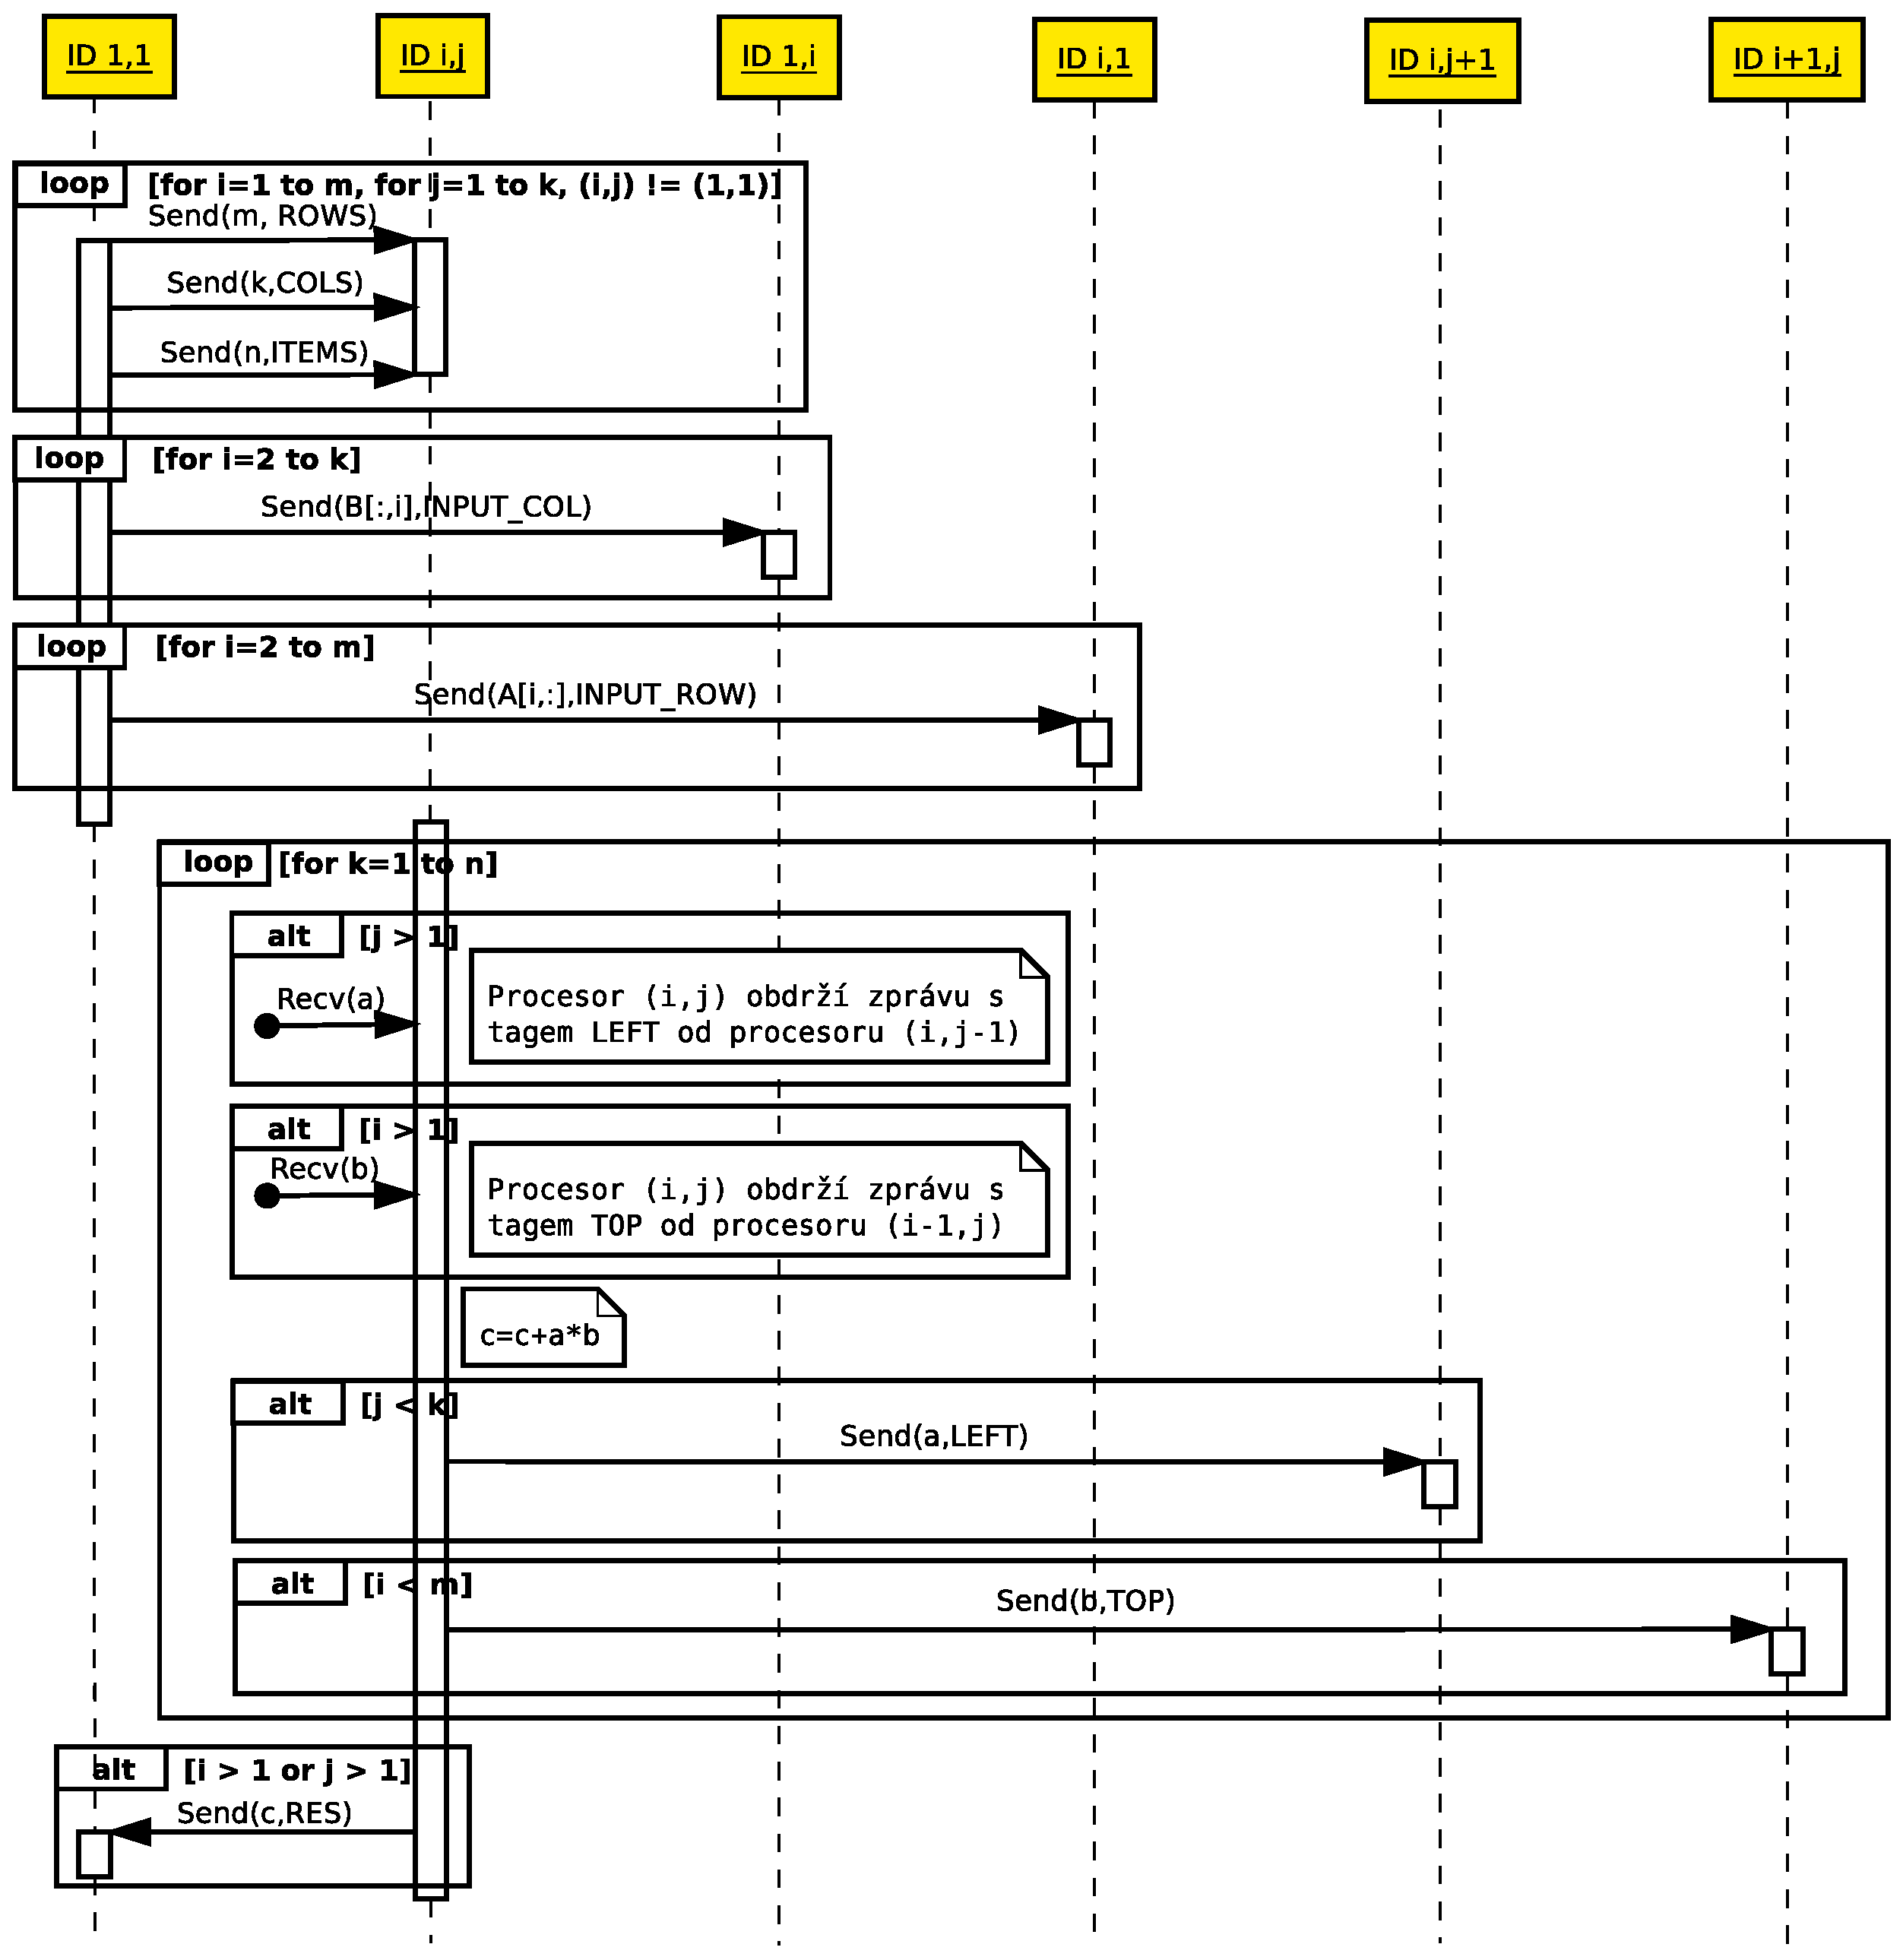
\includegraphics[scale=0.3]{Figures/SequenceDiagram.eps}
  \caption{Komunikační protokol pro násobení matice $\mathbf{A}$ o rozměru $m\times n$ s maticí $\mathbf{B}$ o rozměru $n\times k$ s 
  využitím $m\cdot k$ procesorů. Zasílání zpráv je označeno plnou šipkou s popisem Send($Hodnota$, $Tag$), kde $Hodnota$ 
  je posílaná hodnota a $Tag$ je zkratka označení zprávy. Pomocí šipky s kulatým koncem s nápisem Recv($x$) je 
  znázorněno přijetí zprávy s hodnotou $x$ (zpráva byla odeslána již dříve). Pomocí notace $\mathbf{A}[:,i]$ je označen $i$-tý sloupec matice $\mathbf{A}$. 
  Podobně $\mathbf{A}[i,:]$ je $i$-tý řádek matice~$\mathbf{A}$.}
  \label{fig:seq}
\end{figure}


\end{document}	
